\chapter{Implementation and Testing}

\section{Functionality Implementation and Test Cases}

This section details the implementation of each major functionality of the MySupplyCo application, along with the corresponding test cases used to validate correct behaviour.

\subsection{User Authentication Functionality}

\textbf{Input:}
\begin{itemize}
    \item User's full name (registration only).
    \item Mobile phone number (10 digits, Indian format with +91 prefix).
    \item One-Time Password (OTP) received via SMS.
    \item Alternatively, Google account credentials for OAuth sign-in.
\end{itemize}

\textbf{Output:}
\begin{itemize}
    \item Successful registration creates a new entry in the \texttt{user\_details} table.
    \item Successful login establishes an authenticated session and redirects to the Home Page.
    \item Guest mode allows unauthenticated read-only access to stock information.
\end{itemize}

\textbf{Process:}
\begin{enumerate}
    \item \textbf{Registration Flow:} User enters full name and mobile number on the Register tab. The system sends an OTP via Supabase Auth (\texttt{signInWithOtp}). User enters the received OTP. The system verifies the OTP (\texttt{verifyOTP}) and creates a user profile in the \texttt{user\_details} table via upsert. The user's preferred language is synced to the backend.

    \item \textbf{Login Flow:} User enters their registered mobile number on the Login tab. OTP is sent and verified. The system checks if a profile exists in \texttt{user\_details}. If found, the user is redirected to the Home Page. If not found, the user is prompted to register first.

    \item \textbf{Google OAuth Flow:} User taps ``Continue with Google''. The system initiates OAuth via \texttt{signInWithOAuth} with a deep link callback (\texttt{supplyco://login-callback/}). On the Register tab, a new profile is created with the entered name and Google email. On the Login tab, existing profiles are verified before granting access.

    \item \textbf{Guest Mode:} User taps ``Continue as Guest'' on the onboarding screen. The system sets a local flag via \texttt{StorageService.setGuestMode(true)} and grants read-only access to stock viewing features without authentication.
\end{enumerate}

\textbf{Test Cases:}
\begin{enumerate}
    \item \textbf{Input:} Valid name and 10-digit phone number, correct OTP. \textbf{Expected Output:} User is registered, profile saved to database, redirected to Home Page.

    \item \textbf{Input:} Phone number with fewer than 10 digits. \textbf{Expected Output:} Error message ``Please enter a valid 10-digit mobile number'' displayed.

    \item \textbf{Input:} Correct phone number but incorrect OTP. \textbf{Expected Output:} Authentication error message displayed, user remains on Auth Page.

    \item \textbf{Input:} Login attempt with unregistered phone number. \textbf{Expected Output:} Message ``Number not registered'' displayed, user redirected to Register tab.

    \item \textbf{Input:} Google Sign-In on Register tab without entering name. \textbf{Expected Output:} Error message ``Please enter your name before continuing with Google''.

    \item \textbf{Input:} Guest mode selection. \textbf{Expected Output:} User can view stores and stock but cannot access notification subscriptions.
\end{enumerate}

\subsection{Store Discovery Functionality}

\textbf{Input:}
\begin{itemize}
    \item Search query (store name or partial name).
    \item District selection from dropdown filter.
    \item GPS coordinates (for nearby store discovery).
\end{itemize}

\textbf{Output:}
\begin{itemize}
    \item List of matching SupplyCo stores with name, district, and address.
    \item Nearby stores ordered by geographical distance.
\end{itemize}

\textbf{Process:}
\begin{enumerate}
    \item \textbf{Search:} User types a store name in the search bar. The system performs client-side filtering on the cached store list, showing real-time suggestions as the user types. Pressing the search button or selecting ``View all'' navigates to a full results page.

    \item \textbf{District Filter:} User selects a district from the dropdown menu populated with all Kerala districts. The store list is filtered to show only outlets in the selected district.

    \item \textbf{Nearby Stores:} The system requests GPS permissions via \texttt{LocationService}. On permission grant, the current position is obtained via \texttt{Geolocator.getCurrentPosition()} with high accuracy. The coordinates are sent to the \texttt{get\_nearby\_stores} RPC function, which returns stores ordered by distance.
\end{enumerate}

\textbf{Test Cases:}
\begin{enumerate}
    \item \textbf{Input:} Search query ``Thrissur''. \textbf{Expected Output:} All stores with ``Thrissur'' in their name or address are displayed.

    \item \textbf{Input:} District filter set to ``Ernakulam''. \textbf{Expected Output:} Only stores in Ernakulam district are shown.

    \item \textbf{Input:} GPS location permission granted. \textbf{Expected Output:} Nearby stores displayed with distance information, ordered from nearest to farthest.

    \item \textbf{Input:} GPS permission denied. \textbf{Expected Output:} Appropriate error message displayed, manual search remains functional.

    \item \textbf{Input:} Empty search query. \textbf{Expected Output:} All stores displayed (no filter applied).
\end{enumerate}

\subsection{Stock Viewing Functionality}

\textbf{Input:}
\begin{itemize}
    \item Store selection (tap on a store from the list).
    \item Optional search query within stock items.
\end{itemize}

\textbf{Output:}
\begin{itemize}
    \item Grid view of all stock items with name, quantity, unit, price, item image, and availability status.
    \item Statistics chips showing total items and available items count.
    \item Special offers tab with promotional information.
\end{itemize}

\textbf{Process:}
\begin{enumerate}
    \item User taps on a store from the Home Page. The Stock Page opens with two tabs: ``Stock Items'' and ``Special''.
    \item If cached stock exists for the selected store, it is displayed immediately while a fresh fetch occurs in the background.
    \item The system calls \texttt{SupabaseService.fetchStock(storeId)}, which queries the \texttt{stock} table with a join to the \texttt{items} table.
    \item Fetched data is displayed in a 2-column grid of stock cards, each showing the item image, name, quantity with unit, price in INR, and an availability badge (green for available, red for unavailable).
    \item Successfully fetched data is saved to local cache via \texttt{StorageService.saveStoreSnapshot()}.
    \item If the network request fails, cached data is shown with an ``Offline'' banner indicating the data age.
\end{enumerate}

\textbf{Test Cases:}
\begin{enumerate}
    \item \textbf{Input:} Store with 15 stock items selected. \textbf{Expected Output:} All 15 items displayed in grid view with correct details.

    \item \textbf{Input:} Search query ``rice'' within stock items. \textbf{Expected Output:} Only items containing ``rice'' in their name are displayed.

    \item \textbf{Input:} Store selected while device is offline, with cached data. \textbf{Expected Output:} Cached stock displayed with offline banner showing time since last update.

    \item \textbf{Input:} Store selected while device is offline, no cached data. \textbf{Expected Output:} Error message with empty state placeholder displayed.

    \item \textbf{Input:} Refresh button tapped while online. \textbf{Expected Output:} Stock data refreshed from server, cache updated.
\end{enumerate}

\subsection{Push Notification System}

\textbf{Input:}
\begin{itemize}
    \item Database webhook trigger when stock table is updated.
    \item User's FCM token stored in \texttt{user\_details}.
\end{itemize}

\textbf{Output:}
\begin{itemize}
    \item Push notification on user's device: ``Restock at [Store Name]! [Item Name] is now back in stock.''
\end{itemize}

\textbf{Process:}
\begin{enumerate}
    \item On app launch, \texttt{NotificationService} requests notification permissions from the user.
    \item If authorized, the FCM token is retrieved and saved to the \texttt{user\_details} table in Supabase.
    \item A token refresh listener ensures the token is updated if it changes.
    \item When the \texttt{sync-stock} edge function updates the stock table, the database webhook triggers the \texttt{send-push} edge function.
    \item The \texttt{send-push} function compares the old and new quantity values. If the old quantity was 0 and the new quantity is greater than 0 (restock event), it proceeds.
    \item The function queries for users whose \texttt{last\_selected\_supplyco} matches the store and who have a valid FCM token.
    \item It authenticates with Firebase using a service account JWT and sends personalized notifications via the FCM v1 API.
\end{enumerate}

\textbf{Test Cases:}
\begin{enumerate}
    \item \textbf{Input:} Stock item quantity changes from 0 to 50. \textbf{Expected Output:} Push notification sent to all users subscribed to that store.

    \item \textbf{Input:} Stock quantity changes from 20 to 50. \textbf{Expected Output:} No notification sent (not a restock from zero).

    \item \textbf{Input:} User denies notification permission. \textbf{Expected Output:} No FCM token saved, user does not receive notifications but app remains functional.

    \item \textbf{Input:} User's FCM token expires and is refreshed. \textbf{Expected Output:} New token automatically saved to Supabase via the \texttt{onTokenRefresh} listener.
\end{enumerate}

\subsection{WhatsApp Alert Subscription}

\textbf{Input:}
\begin{itemize}
    \item User's WhatsApp phone number (10 digits).
    \item Selection of commodities to monitor (from a list of 13 items).
    \item Optional ``Notify me about special offers'' checkbox.
\end{itemize}

\textbf{Output:}
\begin{itemize}
    \item Subscription confirmation displayed to the user.
    \item User preferences saved for future WhatsApp alert delivery.
\end{itemize}

\textbf{Process:}
\begin{enumerate}
    \item User navigates to the WhatsApp Alerts page from the Home Page.
    \item User enters their WhatsApp number and selects commodities from the checklist (Rice, Sugar, Coconut Oil, Wheat, Dal variants, Mustard Oil, Salt, Onion, Potato, Tomato, Milk, Atta).
    \item A ``Select All / Deselect All'' toggle is available for convenience.
    \item User taps ``Enable WhatsApp Alerts'' button.
    \item The system validates the phone number (exactly 10 digits, numeric only) and ensures at least one commodity or special offers is selected.
    \item On successful validation, a confirmation is displayed and the user is redirected to the Home Page.
\end{enumerate}

\textbf{Test Cases:}
\begin{enumerate}
    \item \textbf{Input:} Valid 10-digit number, 3 commodities selected. \textbf{Expected Output:} Subscription confirmed, user redirected to Home Page.

    \item \textbf{Input:} Phone number with 8 digits. \textbf{Expected Output:} Error message ``Please enter a valid 10-digit phone number''.

    \item \textbf{Input:} Valid phone number, no commodities selected, special offers unchecked. \textbf{Expected Output:} Error message ``Please select at least one item or special offers''.

    \item \textbf{Input:} ``Select All'' toggled on. \textbf{Expected Output:} All 13 commodity checkboxes become checked.
\end{enumerate}

\subsection{Localization (Multi-Language Support)}

\textbf{Input:}
\begin{itemize}
    \item Language selection from the language dialog or onboarding screen.
\end{itemize}

\textbf{Output:}
\begin{itemize}
    \item Entire application UI dynamically updates to the selected language without requiring a restart.
\end{itemize}

\textbf{Process:}
\begin{enumerate}
    \item On first launch, the onboarding screen presents language options: English (default) and ``Others'' (expanding to show Malayalam, Hindi, Gujarati, Marathi, Bengali, Tamil, Telugu).
    \item Language selection updates \texttt{LocalizationProvider}, which calls \texttt{notifyListeners()} to trigger a reactive UI rebuild.
    \item The selected language code is persisted locally via \texttt{StorageService.setPreferredLanguage(code)}.
    \item For authenticated users, the language preference is synced to the \texttt{user\_details.preferred\_language} column in Supabase.
    \item The \texttt{MaterialApp} widget consumes the locale from the provider and loads the corresponding ARB-generated localization delegates.
\end{enumerate}

\textbf{Test Cases:}
\begin{enumerate}
    \item \textbf{Input:} Language changed from English to Malayalam. \textbf{Expected Output:} All UI strings (buttons, labels, titles, descriptions) display in Malayalam.

    \item \textbf{Input:} Language set to Hindi, app restarted. \textbf{Expected Output:} App launches in Hindi (persisted preference loaded from local storage).

    \item \textbf{Input:} Authenticated user changes language. \textbf{Expected Output:} Language preference synced to Supabase \texttt{user\_details} table.
\end{enumerate}

\subsection{Profile and Settings}

\textbf{Input:}
\begin{itemize}
    \item Navigation to Profile \& Settings page.
    \item User interactions: language change, logout, navigation to sub-pages.
\end{itemize}

\textbf{Output:}
\begin{itemize}
    \item User profile information displayed (name, masked phone number).
    \item Access to settings: language, accessibility, help, terms, privacy policy.
    \item Logout functionality clearing the session.
\end{itemize}

\textbf{Process:}
\begin{enumerate}
    \item On page load, \texttt{\_loadUserDetails()} fetches the user's name, phone number, and language preference from the \texttt{user\_details} table.
    \item The profile card displays the user's name in uppercase with a circular avatar (first letter of name) and a masked phone number (e.g., \texttt{+91******4321}).
    \item Guest users see ``GUEST USER'' with no phone number.
    \item Settings are organized into three groups: Profile/Alerts, Language/Accessibility, and Support/Legal.
    \item The logout button calls \texttt{supabase.auth.signOut()} and navigates to the Auth Page, clearing the navigation stack.
\end{enumerate}

\textbf{Test Cases:}
\begin{enumerate}
    \item \textbf{Input:} Authenticated user opens Profile page. \textbf{Expected Output:} User's name and masked phone number displayed correctly.

    \item \textbf{Input:} Guest user opens Profile page. \textbf{Expected Output:} ``GUEST USER'' displayed, Set Profile option available.

    \item \textbf{Input:} User taps ``Log Out''. \textbf{Expected Output:} Session cleared, user redirected to Auth Page.
\end{enumerate}

\section{Testing Strategies}

The following testing strategies were employed throughout the development of the MySupplyCo application:

\begin{enumerate}
    \item \textbf{Unit Testing:}
    \begin{itemize}
        \item Writing tests for individual service methods (e.g., \texttt{SupabaseService.fetchStock()}, \texttt{StorageService.getTimeAgo()}) to verify correct data transformation and error handling in isolation.
        \item Testing localization helper methods for correct language code mapping.
    \end{itemize}

    \item \textbf{Integration Testing:}
    \begin{itemize}
        \item Testing the interaction between the Flutter application and Supabase backend, verifying authentication flows, data fetching, and profile management end-to-end.
        \item Verifying the sync-stock edge function correctly fetches data from the Django API and upserts it into the Supabase database.
        \item Testing the send-push edge function's restock detection logic and FCM notification delivery.
    \end{itemize}

    \item \textbf{End-to-End Testing:}
    \begin{itemize}
        \item Simulating complete user journeys: from app launch through onboarding, store selection, stock viewing, and notification receipt.
        \item Testing the offline-to-online transition: verifying cached data display, background refresh, and cache update.
    \end{itemize}

    \item \textbf{User Interface Testing:}
    \begin{itemize}
        \item Ensuring UI consistency and responsiveness across different Android screen sizes and densities.
        \item Verifying that all eight language translations render correctly without text overflow or layout issues.
        \item Testing accessibility features including color contrast and touch target sizes.
    \end{itemize}

    \item \textbf{Location-Based Testing:}
    \begin{itemize}
        \item Testing GPS permission flows (granted, denied, permanently denied) on physical devices.
        \item Verifying the accuracy of nearby store results using known GPS coordinates.
        \item Testing behaviour when location services are disabled at the device level.
    \end{itemize}
\end{enumerate}

\section{Source Code}

The complete source code for the MySupplyCo project is available on GitHub:

\begin{center}
\url{https://github.com/Abhinand-Ullas/Supply_co_app}
\end{center}

The repository contains:
\begin{itemize}
    \item Flutter mobile application source code (\texttt{lib/} directory)
    \item Supabase Edge Functions (\texttt{lib/supabase\_backend/})
    \item Localization files for 8 languages (\texttt{lib/generated\_localizations/})
    \item Asset files including app logo and launcher images (\texttt{lib/images/})
    \item Configuration files (\texttt{pubspec.yaml}, \texttt{l10n.yaml}, \texttt{analysis\_options.yaml})
\end{itemize}

\section{Screenshots}

The following screenshots demonstrate the key screens of the MySupplyCo mobile application.

% ─── Placeholder Screenshots (Replace with actual images) ───
% To replace: save your screenshot PNGs in the images/ folder
% and change \fbox{...} to \includegraphics[width=0.45\textwidth]{filename}

\begin{figure}[H]
\centering
\begin{minipage}{0.45\textwidth}
\centering
\fbox{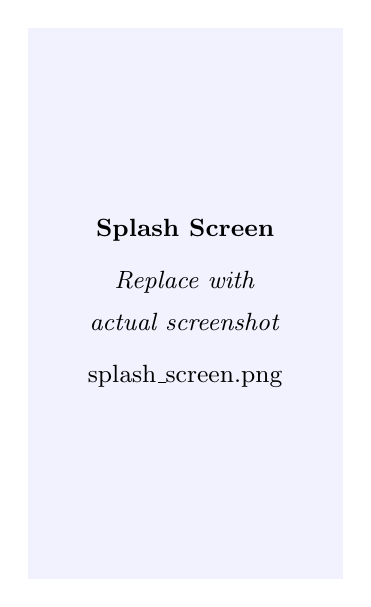
\begin{tikzpicture}
\fill[blue!5] (0,0) rectangle (4,7);
\node[align=center, font=\small] at (2,3.5) {\textbf{Splash Screen}\\[8pt]\textit{Replace with}\\[4pt]\textit{actual screenshot}\\[8pt]splash\_screen.png};
\end{tikzpicture}}
\caption{Splash Screen}
\label{fig:splash}
\end{minipage}
\hfill
\begin{minipage}{0.45\textwidth}
\centering
\fbox{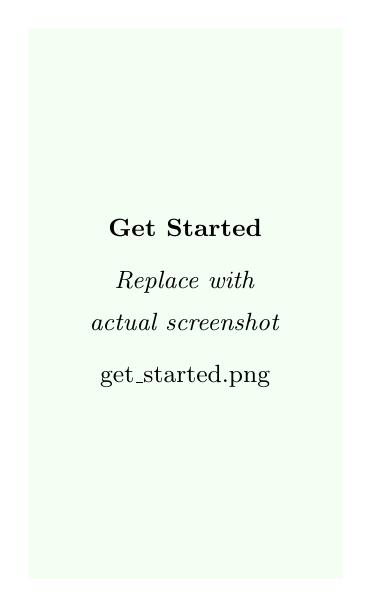
\begin{tikzpicture}
\fill[green!5] (0,0) rectangle (4,7);
\node[align=center, font=\small] at (2,3.5) {\textbf{Get Started}\\[8pt]\textit{Replace with}\\[4pt]\textit{actual screenshot}\\[8pt]get\_started.png};
\end{tikzpicture}}
\caption{Get Started / Onboarding Screen}
\label{fig:getstarted}
\end{minipage}
\end{figure}

\begin{figure}[H]
\centering
\begin{minipage}{0.45\textwidth}
\centering
\fbox{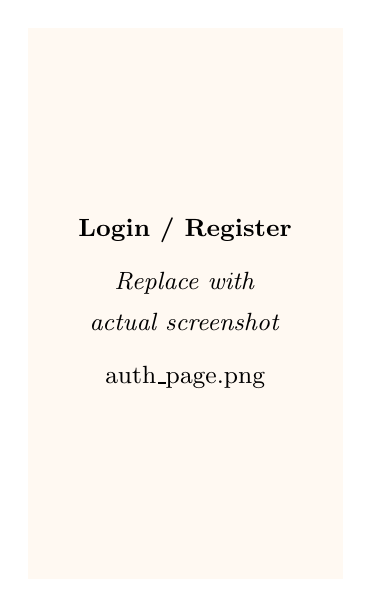
\begin{tikzpicture}
\fill[orange!5] (0,0) rectangle (4,7);
\node[align=center, font=\small] at (2,3.5) {\textbf{Login / Register}\\[8pt]\textit{Replace with}\\[4pt]\textit{actual screenshot}\\[8pt]auth\_page.png};
\end{tikzpicture}}
\caption{Login / Register Screen}
\label{fig:auth}
\end{minipage}
\hfill
\begin{minipage}{0.45\textwidth}
\centering
\fbox{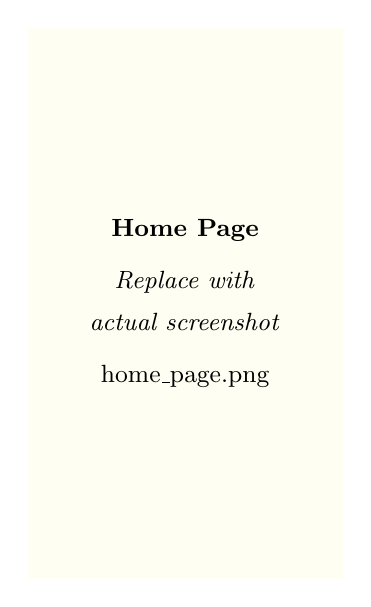
\begin{tikzpicture}
\fill[yellow!5] (0,0) rectangle (4,7);
\node[align=center, font=\small] at (2,3.5) {\textbf{Home Page}\\[8pt]\textit{Replace with}\\[4pt]\textit{actual screenshot}\\[8pt]home\_page.png};
\end{tikzpicture}}
\caption{Home Page with Store Listing}
\label{fig:home}
\end{minipage}
\end{figure}

\begin{figure}[H]
\centering
\begin{minipage}{0.45\textwidth}
\centering
\fbox{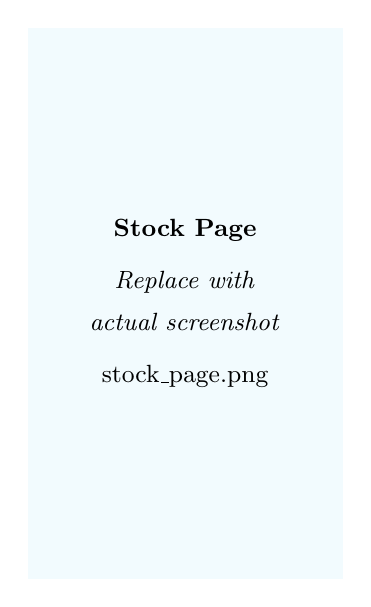
\begin{tikzpicture}
\fill[cyan!5] (0,0) rectangle (4,7);
\node[align=center, font=\small] at (2,3.5) {\textbf{Stock Page}\\[8pt]\textit{Replace with}\\[4pt]\textit{actual screenshot}\\[8pt]stock\_page.png};
\end{tikzpicture}}
\caption{Stock Page with Item Grid}
\label{fig:stock}
\end{minipage}
\hfill
\begin{minipage}{0.45\textwidth}
\centering
\fbox{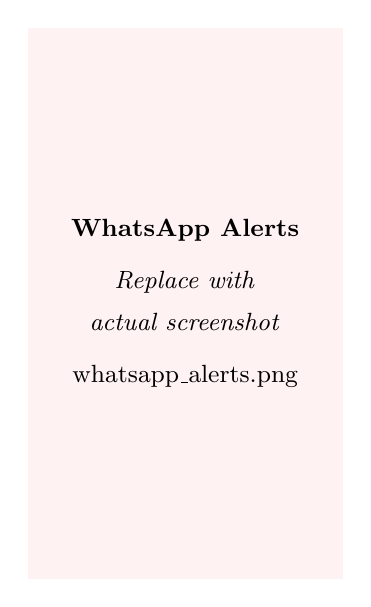
\begin{tikzpicture}
\fill[red!5] (0,0) rectangle (4,7);
\node[align=center, font=\small] at (2,3.5) {\textbf{WhatsApp Alerts}\\[8pt]\textit{Replace with}\\[4pt]\textit{actual screenshot}\\[8pt]whatsapp\_alerts.png};
\end{tikzpicture}}
\caption{WhatsApp Alert Subscription Page}
\label{fig:whatsapp}
\end{minipage}
\end{figure}

\begin{figure}[H]
\centering
\begin{minipage}{0.45\textwidth}
\centering
\fbox{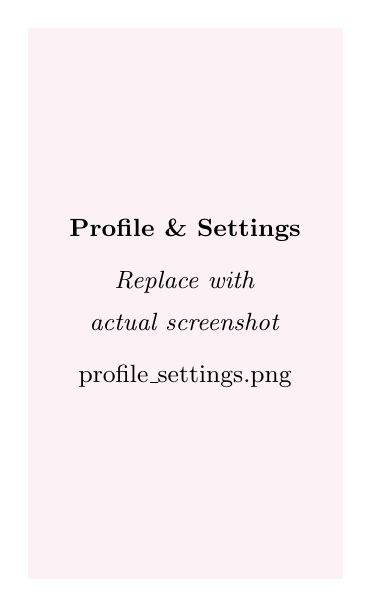
\begin{tikzpicture}
\fill[purple!5] (0,0) rectangle (4,7);
\node[align=center, font=\small] at (2,3.5) {\textbf{Profile \& Settings}\\[8pt]\textit{Replace with}\\[4pt]\textit{actual screenshot}\\[8pt]profile\_settings.png};
\end{tikzpicture}}
\caption{Profile and Settings Page}
\label{fig:profile}
\end{minipage}
\hfill
\begin{minipage}{0.45\textwidth}
\centering
\fbox{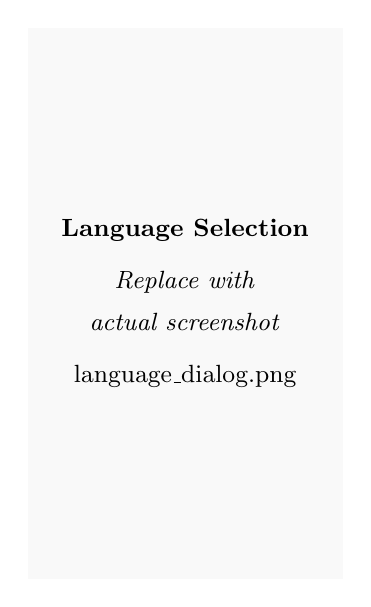
\begin{tikzpicture}
\fill[gray!5] (0,0) rectangle (4,7);
\node[align=center, font=\small] at (2,3.5) {\textbf{Language Selection}\\[8pt]\textit{Replace with}\\[4pt]\textit{actual screenshot}\\[8pt]language\_dialog.png};
\end{tikzpicture}}
\caption{Language Selection Dialog}
\label{fig:language}
\end{minipage}
\end{figure}
